\section{Sharding}


En el ejercicio 7, nos piden experimentar con sharding.
Para esto decidimos tomar como base 3 mil registros de la tabla Competidor, y luego realizar la partición en 3 shards.
Generamos inserts cada 100 competidores, y registramos los resultado evaluados en los shard.
Los datos obtenidos esta plasmados en el siguiente gráfico:

\begin{center}
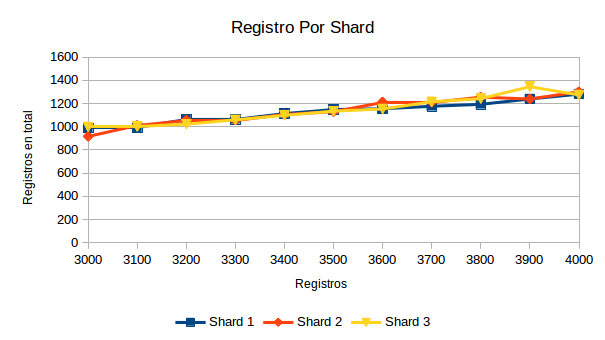
\includegraphics[width=11cm,keepaspectratio]{./imagenes/shard.png}\newline
\end{center}

Se puede ver que la distribución de los datos es uniforme, de manera tal de no sobrecargar la base al realizar consultas y\/o modificaciones.